\chapter{Electrical Foundations: CMOS, Outputs, and Buses}
\label{ch:electrical}

We have followed the design all the way from text to a bitstream on the board,
and the ``Security Panel'' machine waits for a code, watches the
door sensor, and switches on the siren. All this time we talked about zeros and
ones as if a signal lived in an ideal world. But the door sensor is a button with
contacts, the siren is an LED or a buzzer, and there are wires between them and the
circuit. Here the idealization stops working: a chip pin gives and takes
\emph{current}, ``0'' and ``1'' are \emph{voltage ranges}, and no
element is isolated from its neighbors. The question of this chapter: what really happens
at the boundary between the chip and the outside world, and what must be added to the circuit so that it
works correctly with buttons, LEDs, and shared lines?

To answer it, we have to look inside a logic gate, examine
levels and currents, and go through three ways of putting a signal on a wire. The chapter is short
and practical: it exists so that the project stops being ``on paper only''.

\begin{buildbox}
The \emph{Learn} tab, the ``Circuits and the board'' book, the ``Connecting to the board'' chapter, the lesson
``An LED and current limiting''. Put an LED on the Lab bench,
connect it to the board, and see what the lesson says about the resistor: why
it is needed and what current is considered safe. Write down what resistor
you think would suit a 3.3~V supply and a current of about 8~mA---in the section
``Load, current, and delay'' we will calculate it.
\end{buildbox}

\section{The Transistor and CMOS Gates}

\subsection{The Transistor as a Switch}

Modern digital circuits are built from field-effect transistors of the \term{MOS}
type (metal--oxide--semiconductor, MOSFET). For our purposes a transistor can be
pictured as a controlled switch with three terminals: the gate (the control terminal),
the source, and the drain (current flows between them).

\begin{itemize}
  \item An \textbf{n-channel} transistor (nMOS) conducts when the gate is
        \emph{high} (1) and breaks the circuit when it is low.
  \item A \textbf{p-channel} transistor (pMOS) works the other way round: it
        conducts when the gate is \emph{low} and is off when it is high.
\end{itemize}

\subsection{The CMOS Inverter}

If we connect both transistors as shown in Figure~\ref{fig:cmos_inv}, we get an
inverter. The pMOS is connected to the supply $U_{\text{DD}}$, the nMOS to ground. The gates
are tied together and form the input, and the connected drains form the output.

\begin{figure}[H]
\centering
\begin{tikzpicture}[font=\sffamily\small, sw/.style={draw, minimum width=11mm, minimum height=9mm, fill=white, rounded corners=1pt}]
  \draw (0,3.4) -- (0,3.8) node[above] {$U_{\text{DD}}$};
  \node[sw] (p) at (0,2.7) {pMOS};
  \node[sw] (n) at (0,0.9) {nMOS};
  \draw (0,3.4) -- (p.north);
  \draw (p.south) -- (0,1.8) -- (n.north);
  \draw (0,1.8) -- (1.4,1.8) node[right] {output};
  \draw (n.south) -- (0,0) node[below] {ground};
  \draw (-1.4,1.8) node[left] {input} -- (-0.85,1.8) -- (-0.85,2.7) -- (p.west);
  \draw (-0.85,1.8) -- (-0.85,0.9) -- (n.west);
  \fill (-0.85,1.8) circle (1.2pt);
  \fill (0,1.8) circle (1.2pt);
  % table
  \node[align=left, anchor=west] at (3.5,3.6) {Input = 1: nMOS is on, pMOS is off\\{}$\Rightarrow$ output is connected to ground (0)};
  \node[align=left, anchor=west] at (3.5,2.2) {Input = 0: pMOS is on, nMOS is off\\{}$\Rightarrow$ output is connected to the supply (1)};
  \node[align=left, anchor=west, text=FpgaGreen!50!black] at (3.5,0.6) {In any steady state exactly one\\transistor is on: there is no current\\from the supply to ground.};
\end{tikzpicture}
\caption{A CMOS inverter: a pair of transistors, one of which is always off}
\label{fig:cmos_inv}
\end{figure}

The main advantage of \term{CMOS} (complementary MOS) is that at rest the circuit
consumes almost no power: there is no path from the supply to ground. Current
appears only at the moment of switching, when the load capacitance and the inputs of
the following gates have to be charged or discharged. That is why the power consumption
is proportional to the frequency.

\begin{ideabox}
The power a CMOS circuit spends on switching is
$P \approx C\cdot U^2\cdot f$, where $C$ is the total capacitance of the switched
nodes, $U$ is the supply voltage, and $f$ is the switching frequency. To
reduce the power, lower the voltage (it is squared!),
the frequency, or the number of switching nodes. That is exactly why in digital circuits
it is a good habit not to clock what is not working.
\end{ideabox}

\subsection{NAND and NOR Gates}

To build a gate with two inputs, transistors are added following
the principle of duality. In a \term{NAND} gate two nMOS transistors are in
series (the path to ground closes only if both inputs are 1), and
two pMOS transistors are in parallel (a single zero is enough to connect the output to
the supply). A \term{NOR} gate is the opposite: the nMOS transistors are in parallel and the pMOS transistors
in series.

\begin{figure}[H]
\centering
\begin{tikzpicture}[font=\sffamily\small, sw/.style={draw, minimum width=9mm, minimum height=8mm, fill=white, rounded corners=1pt}]
  % NAND
  \node at (1.5,4.9) {\textbf{NAND}};
  \draw (1.5,4.5) -- (1.5,4.2) node[above, yshift=-2pt] {};
  \draw (0.4,4.2) -- (2.6,4.2);
  \node[sw] (p1) at (0.4,3.4) {p};
  \node[sw] (p2) at (2.6,3.4) {p};
  \draw (0.4,4.2) -- (p1.north); \draw (2.6,4.2) -- (p2.north);
  \draw (0.4,3.0) -- (0.4,2.7) -- (2.6,2.7) -- (2.6,3.0);
  \draw (1.5,2.7) -- (3.4,2.7) node[right] {$Y$};
  \node[sw] (n1) at (1.5,1.9) {n};
  \node[sw] (n2) at (1.5,0.7) {n};
  \draw (1.5,2.7) -- (n1.north); \draw (n1.south) -- (n2.north); \draw (n2.south) -- (1.5,0.2) node[below] {ground};
  \node[left] at (-0.3,3.4) {$A$}; \node[left] at (0.9,1.9) {$A$}; \node[right] at (3.2,3.4) {$B$}; \node[left] at (0.9,0.7) {$B$};
  % NOR
  \begin{scope}[xshift=7.5cm]
  \node at (1.5,4.9) {\textbf{NOR}};
  \node[sw] (q1) at (1.5,4.0) {p};
  \node[sw] (q2) at (1.5,2.8) {p};
  \draw (1.5,4.6) -- (q1.north); \draw (q1.south) -- (q2.north);
  \draw (1.5,2.4) -- (1.5,2.0);
  \draw (1.5,2.0) -- (3.4,2.0) node[right] {$Y$};
  \draw (0.4,2.0) -- (2.6,2.0);
  \node[sw] (m1) at (0.4,1.2) {n};
  \node[sw] (m2) at (2.6,1.2) {n};
  \draw (0.4,2.0) -- (m1.north); \draw (2.6,2.0) -- (m2.north);
  \draw (0.4,0.8) -- (0.4,0.3) -- (2.6,0.3) -- (2.6,0.8);
  \draw (1.5,0.3) -- (1.5,0.0) node[below] {ground};
  \node[left] at (0.9,4.0) {$A$}; \node[left] at (0.9,2.8) {$B$}; \node[left] at (-0.0,1.2) {$A$}; \node[right] at (3.1,1.2) {$B$};
  \end{scope}
\end{tikzpicture}
\caption{Circuits of CMOS gates. Only the transistors and connections are shown; gates labeled with the same letter are connected to each other. The supply is connected to the top terminal}
\label{fig:cmos_nand}
\end{figure}

That is why in CMOS the ``basic'' gates are inverting. For an AND gate
you have to add an inverter (six transistors in total instead of four). For
exactly this reason in Chapter~\ref{ch:gates} we called NAND and NOR universal and
economical: they are also physically simpler.

\begin{diybox}[A Gate Built from Gates]
\textbf{Task.} Check that NAND really is simpler than AND, and build NAND
as the chain ``AND, then NOT''.\\
\textbf{In Logra.} The \emph{Learn} tab, the ``Circuits and the board'' book, the ``Logic
gates'' chapter: the lesson ``NAND from blocks''; the \emph{Designer} and
\emph{Waveforms} tabs.\\
\stars{1} \emph{Repeat.} Build NAND from blocks and check the four rows of the
truth table.\\
\stars{2} \emph{Modify.} Build AND as ``NAND, then NOT'' and count the
transistors using Figures~\ref{fig:cmos_inv} and~\ref{fig:cmos_nand}: in CMOS
NAND has 4 of them, AND has 6 (NAND and an inverter).\\
\stars{3} \emph{Project.} Problem~1: draw a CMOS circuit of a three-input NOR and
state the number of transistors of each type.\\
\textbf{Expected result.} The waveforms of the ``NAND'' and ``AND + NOT'' circuits are identical;
the number of transistors for ``AND'' is larger than for ``NAND''.\\
\textbf{How to check.} The \emph{Waveforms} tab: go through the four combinations;
the \emph{RTL} tab: compare the number of elements.
\end{diybox}

\section{Signal Levels and Noise Margin}

A real output does not deliver ``exactly zero'' and ``exactly the supply'': it
guarantees only that a 0 will be no higher than $U_{OL}$, and a 1 no lower than
$U_{OH}$. An input, in turn, treats everything not higher than $U_{IL}$ as low, and
everything not lower than $U_{IH}$ as high. Between them lies a forbidden zone.

\begin{table}[H]
\centering
\caption{Typical thresholds for 3.3~V logic (LVTTL/LVCMOS33)}
\small
\begin{tabular}{llr}
\toprule
\textbf{Parameter} & \textbf{Meaning} & \textbf{Value} \\
\midrule
$U_{OL}$ & output at 0, at most & 0.4~V \\
$U_{OH}$ & output at 1, at least & 2.4~V \\
$U_{IL}$ & input reads 0 if at most & 0.8~V \\
$U_{IH}$ & input reads 1 if at least & 2.0~V \\
\bottomrule
\end{tabular}
\end{table}

The noise margin is the difference between what the output guarantees and what
the input requires: $N_L = U_{IL}-U_{OL} = 0.4$~V for zero and
$N_H = U_{OH}-U_{IH} = 0.4$~V for one. Interference smaller than these values
will not spoil the signal. This is exactly why a digital circuit is so robust: as long as the interference
is smaller than the margin, the signal is ``cleaned up'' at every gate.

\begin{diybox}[Levels and Threshold]
\textbf{Task.} Find out what supply voltage and what thresholds the board pins
have, and estimate the noise margin.\\
\textbf{In Logra.} The \emph{Pins} tab: choose any port and find in its
card the standard and the voltage (it shows LVCMOS33, 3.3~V); the
\emph{Waveforms} tab.\\
\stars{1} \emph{Repeat.} Write out for the port the thresholds $U_{OL}$, $U_{OH}$,
$U_{IL}$, $U_{IH}$ from the table in this chapter and find the margins $N_L$ and $N_H$.\\
\stars{2} \emph{Modify.} Suppose a sensor applies 1.4~V to a port input. Which
way will the chip read it? What would you do to prevent that?
(Problem~4)\\
\stars{3} \emph{Project.} One of the panel sensors outputs 5~V. Explain why
it cannot be connected directly to a 3.3~V port, and suggest protection (a divider of
two resistors).\\
\textbf{Expected result.} For a 3.3~V input, everything at or above 2.0~V counts as one, and everything at or below 0.8~V
counts as zero.\\
\textbf{How to check.} Compare with the table in this chapter and with the port card in the
\emph{Pins} tab; check the margin calculation against the answer to Problem~4.
\end{diybox}

\section{Load, Current, and Delay}

The output of a gate is connected to the inputs of the following gates, each of which
has a small capacitance, plus the wire itself. The larger the capacitance, the longer the output
takes to go from 0 to 1, and the larger the delay. The number of inputs that one output can
drive is called the \term{fan-out}. This
is clearly visible in the frequency report: a signal that goes to a hundred inputs (for example,
reset) is slower than a signal that goes to one.

\subsection{Output Current and the LED Resistor}

For chip pins the main limitation is current. An LED requires
a few milliamps, and a port is rated for a limited current (in our case
up to 8~mA). You cannot connect a heavy load (a motor, a relay) to a pin: you need
an amplifier built from a transistor. But an LED also must not be connected directly to an output:
its resistance in the on state is almost zero, and the current grows to
dangerous values. That is why a resistor is placed in series with the LED
to set the current:
\[
  R = \frac{U_\text{DD} - U_\text{LED}}{I}.
\]
Here $U_\text{LED}$ is the voltage that ``drops'' across the LED in the
on state (about 2~V for a red one). Example: supply 3.3~V, drop across the
LED 2.0~V, required current 8~mA. Then
$R = (3.3-2.0)/0.008 \approx 163$~$\Omega$. We take the nearest larger
standard value from the series: 180~$\Omega$. The current is then
$I = 1.3/180 \approx 7.2$~mA, slightly less than intended, but safe.

In a project the port current limit is set in the constraints file with the
parameter \code{DRIVE=8}, and the resistor is taken on the board; an example
file is at the end of the section ``Pull-Ups and Pull-Downs'' and in
Chapter~\ref{ch:bridge}.

\begin{diybox}[A Resistor for an LED]
\textbf{Task.} Choose a resistor for an LED and see that without
it the circuit is ``wrong''.\\
\textbf{In Logra.} The \emph{Learn} tab, the ``Circuits and the board'' book, the chapter
``Connecting to the board'': the lesson ``An LED and current limiting''; the
\emph{Lab} tab.\\
\stars{1} \emph{Repeat.} Put an LED on the Lab bench and connect
it to the board following the lesson.\\
\stars{2} \emph{Modify.} Calculate the resistor for a green LED
($U_\text{LED}=2.2$~V) at a 3.3~V supply and a current of 5~mA, and check the calculation
with the formula of this chapter.\\
\stars{3} \emph{Project.} \textbf{A stage of the ``Security Panel'' project:} the
siren indicator. Draw the circuit that connects the ``ALARM'' LED to a port and choose a
resistor. Acceptance criterion: the current is at most 8~mA, the power in the resistor is at
most 0.25~W, and the circuit states the value and the series.\\
\textbf{Expected result.} For 3.3~V and 5~mA you get about 220~$\Omega$.\\
\textbf{How to check.} Compare with the answer to Problem~8; in the Lab the LED
should light steadily, without overload.
\end{diybox}

\section{Outputs, Buses, and Three States}

\subsection{Types of Outputs}

Digital technology uses three different output circuits.

\begin{figure}[H]
\centering
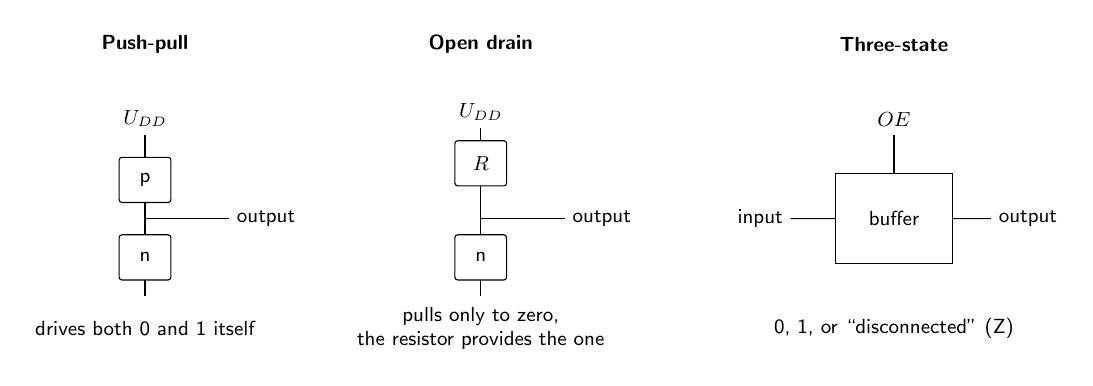
\begin{tikzpicture}[scale=0.82, transform shape, font=\sffamily\small, sw/.style={draw, minimum width=8mm, minimum height=7mm, fill=white, rounded corners=1pt}]
  % Push-pull
  \node at (0,4.6) {\textbf{Push-pull}};
  \draw (0,3.2) -- (0,3.0);
  \node[sw] (a) at (0,2.5) {p}; \node[sw] (b) at (0,1.3) {n};
  \draw (0,3.2) node[above] {$U_{\text{DD}}$} -- (a.north); \draw (a.south) -- (b.north); \draw (0,1.9) -- (1.3,1.9) node[right] {output}; \draw (b.south) -- (0,0.7) node[below] {};
  \node[align=center] at (0,0.2) {drives both 0 and 1 itself};
  % Open drain
  \begin{scope}[xshift=5.2cm]
  \node at (0,4.6) {\textbf{Open drain}};
  \node[sw] (c) at (0,1.3) {n};
  \draw (0,1.9) -- (c.north); \draw (0,1.9) -- (1.3,1.9) node[right] {output}; \draw (c.south) -- (0,0.7);
  \draw (0,1.9) -- (0,2.4) node[sw, anchor=south] {$R$} ; \draw (0,3.1) -- (0,3.3) node[above] {$U_{\text{DD}}$};
  \node[align=center] at (0,0.2) {pulls only to zero,\\the resistor provides the one};
  \end{scope}
  % Three-state
  \begin{scope}[xshift=11.6cm]
  \node at (0,4.6) {\textbf{Three-state}};
  \node[draw, minimum width=18mm, minimum height=14mm, fill=white] (t) at (0,1.9) {buffer};
  \draw (-1.6,1.9) node[left] {input} -- (t.west);
  \draw (t.east) -- (1.5,1.9) node[right] {output};
  \draw (0,3.2) node[above] {$OE$} -- (t.north);
  \node[align=center] at (0,0.2) {0, 1, or ``disconnected'' (Z)};
  \end{scope}
\end{tikzpicture}
\caption{Three output circuits of digital gates}
\end{figure}

\begin{itemize}
  \item A \textbf{push-pull} output actively drives both 0 and 1. Such
        outputs are on most chip pins.
  \item An \textbf{open-drain} output can only connect the output to
        ground. The one is created by an external pull-up resistor. But any number of such outputs
        can be connected to one line: the line will be at
        zero if \emph{at least one} pulls it to ground, which gives the
        AND function (``wired AND''). \lookahead{this is how the serial
        I$^2$C bus works (Chapter~\ref{ch:uart}).}
  \item A \textbf{three-state} (tri-state, 3-state) output can drive 0, 1,
        or be \emph{disconnected}: the high-impedance state $Z$. It is the
        disconnectable output that lets several sources take turns
        using a shared wire.
\end{itemize}

\subsection{A Bus with Several Sources}

A \term{bus} is a group of shared wires to which several
devices are connected. At any moment exactly one transmits, and the others must be
disconnected (state $Z$). Choosing the transmitter is the same task that a
multiplexer solves (Chapter~\ref{ch:mux}), only physical: instead of a logical
choice, the output of all but one is simply disconnected from the wire.

\begin{figure}[H]
\centering
\begin{tikzpicture}[font=\sffamily\small]
  \foreach \i/\y in {1/2.4, 2/1.2, 3/0} {
    \node[draw, minimum width=14mm, minimum height=7mm, fill=white] (b\i) at (2,\y) {buffer $\i$};
    \draw (0.1,\y) node[left] {$D_\i$} -- (b\i.west);
    \draw (b\i.east) -- (4.2,\y);
    \node[font=\sffamily\scriptsize] at (2,\y+0.58) {$OE_\i$};
  }
  \draw[very thick] (4.2,-0.4) -- (4.2,2.8);
  \node[anchor=south west, inner sep=2pt] at (4.0,2.8) {shared bus};
  \node[align=left, anchor=west] at (7.0,2.0) {Only one of\\$OE_1, OE_2, OE_3$ is enabled.};
  \node[align=left, anchor=west, text=FpgaRed] at (7.0,0.3) {If two are enabled with different\\data, the outputs ``fight'':\\a short-circuit current.};
\end{tikzpicture}
\caption{Three sources on one bus}
\end{figure}

\begin{warnbox}
If two transmitters are enabled at the same time and drive different values, one pulls the
line to the supply and the other to ground: a large current flows through them, and the line
gets an undefined voltage. This is a \term{bus conflict}. In
simulation it looks like the value \code{X}; on a real board, like
overheating and failure. The control circuit must guarantee that
only one transmitter is enabled at a time.
\end{warnbox}

\subsection{A Three-State Output in Practice}

A three-state output is described by a conditional rule: ``if the output is enabled,
drive the value, otherwise the state $Z$''. A bidirectional pin adds to
this reading what is actually on the wire, so that the circuit can both
transmit and receive over the same line. In simulation such a
state looks like ``disconnected'' (Z), and in a conflict of two transmitters,
like the undefined value \code{X}.

\begin{infobox}[What Happens Inside a Chip]
Inside the chip there are no shared wires with several transmitters: every
signal is driven by exactly one source, and the choice of source is made by
multiplexers. Three-state elements exist only in the input/output blocks
on the pins. Therefore inside the circuit shared buses with the state $Z$ are not built:
multiplexers are used instead.
\end{infobox}

\subsection{Three States in Verilog}

The state $Z$ is written in Verilog as the value \code{z}. A three-state buffer
is a conditional assignment \code{assign pin = oe ? d : 1'bz;}: when
\code{oe = 1} the line repeats \code{d}, when \code{oe = 0} the circuit
``lets go'' of the wire. Inside the chip there are no shared wires, so a bus of
several sources is built there on a multiplexer: it chooses exactly one source.

\vfile{\codepath/b5a_electrical/tristate.v}{code/b5a\_electrical/tristate.v}

\textbf{How to read it.} \code{tri\_buf} is one buffer; on RTL it looks like a
separate element with an enable input. In \code{bus\_mux} a single assignment
chooses \code{a} or \code{b}: this is how a bus is arranged \emph{inside} the
chip. Both modules are checked by \code{tb\_tristate.v}.

A shared line with several transmitters, a conflict and an open drain can only
be \emph{simulated}: Yosys does not accept two sources on one wire, and the
chip never has such a thing. So the models live in the testbench
\code{tb\_bus.v} and run in Icarus Verilog. It has three models: a bus of two
sources with selection by an address, a bus with \emph{independent} enables
(this must not be done: both can be switched on), and an open-drain output.

\vfile{\codepath/b5a_electrical/tb_bus.v}{code/b5a\_electrical/tb\_bus.v}

\textbf{How to read it.} In \code{bus\_two} two \code{assign} statements drive
the same wire \code{bus}; this is allowed because at any moment exactly one of
the conditions selects a value and the other gives \code{z}. In \code{bus\_free}
the conditions are independent: with \code{en\_a = en\_b = 1} and different data
the wire becomes \code{x}---in simulation this is exactly a bus conflict. In
\code{open\_drain2} each participant either pulls the line to zero or releases
it; the one comes from an external pull-up that is not in the module itself. The
testbench sets the pull-up with the net \code{tri1 line;}---``a wire with a
resistor to the supply''; without it a free line would stay in state $Z$ instead
of becoming one. The result: the line is 0 if \emph{at least one} participant
pulls down---this is exactly the ``wired AND''.

A bidirectional pin adds reading of what is really on the wire. It is
described by a separate module:

\vfile{\codepath/00_theory/io_pad.v}{code/00\_theory/io\_pad.v}

\shot{n-iopad-rtl}{A bidirectional pin: a three-state buffer on the output and an ordinary level reading on the input}{fig:n-iopad}

RTL (Figure~\ref{fig:n-iopad}) shows the three-state buffer on the output and an
ordinary read line. Inside the circuit itself this is not done: the three-state
stays at the edge of the chip, where there is physically a shared pin.

\begin{diybox}[Three States and a Conflict]
\textbf{Task.} See the three output states and a conflict on a shared line.\\
\textbf{In Logra.} The \emph{Code} tab, a new project; the \emph{Waveforms} tab.\\
\stars{1} \emph{Repeat.} Describe a three-state buffer:
\code{assign pin = oe ? d : 1'bz;} --- and in \emph{Waveforms} apply $oe=0$,
then $oe=1$ with $d=0$ and $d=1$: find the Z state in the waveform.\\
\stars{2} \emph{Modify.} Add a second buffer to the same line with
\code{oe2} and data $d_2$ in the testbench (in Logra two sources on one wire do
not build: Yosys does not accept it); enable both with different data and find the
value \code{X}.\\
\stars{3} \emph{Project.} A device for two door sensors on one line:
each sensor is connected through its own buffer with an enable; write the condition
that guarantees that only one is enabled at a time. Acceptance
criterion: for any combination of inputs there is no value \code{X} (in the
testbench for the line model, on a waveform for the multiplexer version).\\
\textbf{Expected result.} At $oe=0$ the line is disconnected (Z); at $oe=1$ it
follows $d$; with two buffers enabled with different data you get \code{X}.\\
\textbf{How to check.} The \emph{Waveforms} tab: three levels (0, 1, Z) on
one line; the \emph{RTL} tab: a buffer with an enable looks like a separate
element.\\
\textbf{The same as a file.} The \emph{Code} tab: paste \code{tristate.v},
``Synthesize'', make \code{tri\_buf} the top module, and on Waveforms apply
$oe = 0$, then $oe = 1$, and find Z. The conflict is shown by the testbench:
\code{iverilog -g2012 -o tb tb\_bus.v tristate.v}, then \code{vvp tb} prints
\code{bus: OK}; in it, with \code{en\_a = en\_b = 1} the wire is \code{x}. Sample
answer to \stars{3}: on the chip the condition ``only one at a time'' holds by
itself if the source is chosen by a multiplexer and not by two independent
enables.
\end{diybox}

\begin{vcode}
module door_line (
    input  sel,                 // 0 --- sensor A talks, 1 --- sensor B talks
    input  door_a, door_b,
    output line
);
    assign line = sel ? door_b : door_a;   // one source at any moment
endmodule
\end{vcode}


\section{Pull-Ups and Pull-Downs}

An input that is not connected to anything ``floats'': its level is determined by
interference, and the circuit may behave randomly. That is why every input needs a
resistor that sets the default level: a \term{pull-up} (to the supply)
or a \term{pull-down} (to ground). In chips such resistors are
often built in. For a button that shorts to ground, a pull-up is needed, and
for a button that shorts to the supply, a pull-down. Then ``not pressed'' gives a
defined level.

The value of a pull resistor is a compromise. The smaller the resistance, the faster the
line returns to one after the button is released (time constant
$\tau = RC$, where $C$ is the line capacitance), but the larger the current that flows while the
button is pressed ($I = U_\text{DD}/R$). For example, for a 100~pF line with a
10~k$\Omega$ resistor, $\tau = 1$~\textmu s, and the current at a press is $3.3/10\,000 \approx
0.33$~mA.

\subsection{A Pull-Up on the Board: The Constraints File}

There is no pull-up in Verilog itself: the module sees only the level at the
input. The pull is enabled in the constraints file \code{.cst}, where each port
is matched with a chip pin and parameters. The parameter \code{PULL\_MODE} takes
the values \code{UP} (a resistor to the supply), \code{DOWN} (to ground) and
\code{NONE}. On the Tang Nano 20K board the buttons \code{S1}, \code{S2} are
already pulled to ground and give 1 when pressed; a button or a switch that
shorts the pin to ground gets a pull to the supply and is then inverted in the
module.

\vfile{\codepath/b5a_electrical/btn_in.v}{code/b5a\_electrical/btn\_in.v}

\begin{vcode}[text]
// A switch to ground: pull-up to the supply, pressed = 0
IO_LOC  "btn_n" 75;                          // pin 75 of header J5
IO_PORT "btn_n" IO_TYPE=LVCMOS33 PULL_MODE=UP;

// Board button S1: pressed = 1, pull-down to ground
IO_LOC  "btn[0]" 88;
IO_PORT "btn[0]" IO_TYPE=LVCMOS33 PULL_MODE=DOWN;
\end{vcode}

The combination ``pull-up $+$ inversion in the module'' reads like this: the pin
is 1 (released), and the module makes a logical one out of the press. The pin
numbers of the buttons and LEDs are taken from the file
\code{code/common/tang\_nano\_20k.cst}, which collects the pins of all the ports of
the book; pin~75 is one of the pins of header J5.

\begin{diybox}[A Button Pull-Up]
\textbf{Task.} Connect a button to a port and see that without a pull
the input ``floats''.\\
\textbf{In Logra.} The \emph{Pins} tab: choose a port for the button and find in
its card the pull selection (none, to~1, to~0); the \emph{Learn} tab, the lesson
``A button controls an LED'' (the chapter ``Connecting to the board'').\\
\stars{1} \emph{Repeat.} Complete the lesson ``A button controls an LED''.\\
\stars{2} \emph{Modify.} For a button that shorts the contact to ground, set
the pull ``to~1''; for a button that shorts to the supply, ``to~0''.\\
\stars{3} \emph{Project.} \textbf{A stage of the ``Security Panel'' project:} a physical
input. Connect a key button and a door sensor (the contact shorts to ground) with
a pull; acceptance criterion: with the button not pressed the input level is
defined (1), when pressed it is 0, and the current drawn by the button is at most
0.5~mA (choose the value using the formula of this section; see also
Problems~9 and~10).\\
\textbf{Expected result.} With the button not pressed the input is one, when
pressed it is zero; the value does not ``wander''.\\
\textbf{How to check.} The \emph{Pins} tab: the pull column of the chosen
port; the \emph{Waveforms} tab: a press gives a clean $1\to0$ transition.\\
\textbf{The same in Verilog.} The \emph{Code} tab: paste \code{btn\_in.v},
``Synthesize''; on the \emph{Pins} tab choose the pull ``to~1'' for the port
\code{btn\_n}. \stars{2} Complete a module for a button that shorts to the
supply (pull to~0): what inversion does it need?\\
\textbf{Sample answer.} A button to the supply gives 1 when pressed, the pull holds
0, so no inversion is needed:
\end{diybox}

\begin{vcode}
module btn_in_vcc (
    input  btn,                  // 0 = released (pull-down), 1 = pressed
    output pressed
);
    assign pressed = btn;
endmodule
\end{vcode}


\begin{warnbox}[Common mistakes]
\begin{itemize}
  \item \textbf{An LED without a resistor.} The current is limited only by the internal
        resistance of the source: the LED or the port fails.
  \item \textbf{A ``floating'' input.} A button without a pull gives random values,
        and the circuit switches itself on and off ``by itself''.
  \item \textbf{Two push-pull outputs on one line.} If they drive different
        values, a short circuit results. A shared line needs open-drain or
        three-state outputs.
  \item \textbf{A pull in the wrong direction.} A button to ground with a pull-down
        always gives 0: pressing is indistinguishable from not pressing.
\end{itemize}
\end{warnbox}

\section{Questions and Problems}
\label{sec:tasks-electrical}

The answers are collected in Appendix~\ref{app:answers}.

\begin{taskbox}[Chapter Problems]
\begin{enumerate}
  \item \stars{2}~Draw a CMOS circuit of a NOR gate with three inputs: how many
        transistors of each type are needed and how are they connected?
  \item \stars{1}~A circuit consumes $P = C U^2 f$. How does the power change if the
        supply is lowered from 3.3~V to 1.8~V with the frequency unchanged?
  \item \stars{1}~Calculate the switching power of a node with a capacitance of 10~pF at a supply of
        3.3~V and a frequency of 27~MHz.
  \item \stars{1}~An output drives 2.6~V, and the input requires at least 2.0~V. What is the noise
        margin for one?
  \item \stars{2}~Why do serial buses with many connected
        devices use open-drain outputs and pull-up
        resistors rather than push-pull outputs?
  \item \stars{1}~What happens if two three-state buffers simultaneously
        drive 0 and 1 onto a shared line?
  \item \stars{2}~\emph{Find the error.} A designer tied together two
        push-pull outputs of two different chips to get an OR function
        of their signals. What is wrong with this circuit, why is it dangerous, and how can it be
        fixed (name two ways)?
  \item \stars{2}~\emph{Design.} The ``ALARM'' LED is driven from a 3.3~V
        port. The voltage drop across the red LED is 2.0~V, the
        required current is 8~mA. Which resistor value from the series 100, 150,
        180, 220, 330~$\Omega$ should you take? What is the current at this value?
  \item \stars{3}~\emph{Mini-project.} Two buttons (both short the line to ground)
        are connected to one line with a shared pull-up to 3.3~V.
        Draw the circuit and determine what function of the presses the
        line performs. Acceptance criterion: a table of all four combinations of presses and
        the line level, and a calculation of the current through the pull-up with both buttons pressed
        for a 10~k$\Omega$ resistor.
  \item \stars{3}~\emph{Mini-project.} A button line has a capacitance of 100~pF.
        The rise time (to 90\,\%) is approximately $2.2\,RC$ and must be at most
        1~\textmu s, and the current with the button pressed must be at most 0.8~mA at a supply of
        3.3~V. Does a suitable pull-up resistor exist? Acceptance criterion:
        the bounds of the value on both sides are found and a conclusion is drawn.
\end{enumerate}
\end{taskbox}

\section{What's Next}

Now the panel can accept a signal from a button and light an LED correctly:
with a pull on the input and a resistor on the output. But an LED is either on or off,
and the world around us is not binary: we need loudness, temperature, brightness. How does a digital
circuit produce the sound of a buzzer at the right frequency, and how does it ``listen'' to an analog
sensor? In Chapter~\ref{ch:analog} we will go through two bridges between the discrete and the
continuous: the DAC/PWM on the output and the ADC on the input.
